\documentclass{article}
\usepackage{amsmath}
\usepackage[mathletters]{ucs}
\usepackage[utf8x]{inputenc}
\usepackage[margin=1.5in]{geometry}
\usepackage{enumerate}
\newtheorem{theorem}{Theorem}
\usepackage[dvipsnames]{xcolor}
\usepackage{pgfplots}
\setlength{\parindent}{0cm}
\usepackage{graphics}
\usepackage{graphicx} % Required for including images
\usepackage{subcaption}
\usepackage{bigintcalc}
\usepackage{pythonhighlight} %for pythonkode \begin{python}   \end{python}
\usepackage{appendix}
\usepackage{arydshln}
\usepackage{physics}
\usepackage{tikz-cd}
\usepackage{booktabs} 
\usepackage{adjustbox}
\usepackage{mdframed}
\usepackage{relsize}
\usepackage{physics}
\usepackage[thinc]{esdiff}
\usepackage{fixltx2e}
\usepackage{esint}  %for lukket-linje-integral
\usepackage{xfrac} %for sfrac
\usepackage{hyperref} %for linker, må ha med hypersetup
\usepackage[noabbrev, nameinlink]{cleveref} % to be loaded after hyperref
\usepackage{amssymb} %\mathbb{R} for reelle tall, \mathcal{B} for "matte"-font
\usepackage{listings} %for kode/lstlisting
\usepackage{verbatim}
\usepackage{graphicx,wrapfig,lipsum,caption} %for wrapping av bilder
\usepackage{mathtools} %for \abs{x}
\usepackage[norsk]{babel}
\definecolor{codegreen}{rgb}{0,0.6,0}
\definecolor{codegray}{rgb}{0.5,0.5,0.5}
\definecolor{codepurple}{rgb}{0.58,0,0.82}
\definecolor{backcolour}{rgb}{0.95,0.95,0.92}
\lstdefinestyle{mystyle}{
    backgroundcolor=\color{backcolour},   
    commentstyle=\color{codegreen},
    keywordstyle=\color{magenta},
    numberstyle=\tiny\color{codegray},
    stringstyle=\color{codepurple},
    basicstyle=\ttfamily\footnotesize,
    breakatwhitespace=false,         
    breaklines=true,                 
    captionpos=b,                    
    keepspaces=true,                 
    numbers=left,                    
    numbersep=5pt,                  
    showspaces=false,                
    showstringspaces=false,
    showtabs=false,                  
    tabsize=2
}

\lstset{style=mystyle}
\author{Oskar Idland}
\title{Eksamen 2019 Høst}
\date{}
\begin{document}
\maketitle
\newpage
\section*{Oppgave 1}
\subsection*{a)}
Ettersom partikler generelt sett har ganske lite energi gir det mening å bruke mindre enheter som eV for energi. For en masseløs partikkel bruker vi $E = mc^2$ for å regne ut bevegelsesmengden $p = mv$. Da får vi at $p = \frac{E}{c^2}v$, men ettersom partikkelen er masseløs gir det oss $v = c$ som da gir $p = \frac{E}{c}$, med enhet $\frac{eV}{c}$.

\subsection*{b)}
For fotoner er energien $E = hν $, hvor frekvensen $ν$ er gitt ved $ν = \frac{c}{λ}$. Setter vi dette inn for energien får vi energien gitt av bølgelengden. 
\[
E = hν = h \frac{c}{λ}
\]
Som forventet øker energien når bølgelengden synker. For et foton med bølgelengde $λ = 5 ⋅ 10^{-7}$ får vi en energi på $E = hc / λ = 1240 \text{ eVnm} / 500 \text{nm} = 2.48 eV$. 
Videre finner vi bevegelsesmengden $p = E / c = 2.48 \text{ eV} / 3 ⋅ 10^{8} \text{ m/s} = 8.27 ⋅ 10^{-9} \text{eV s/m}$

\subsection*{c)}
\begin{figure}[h!]
  \centering
  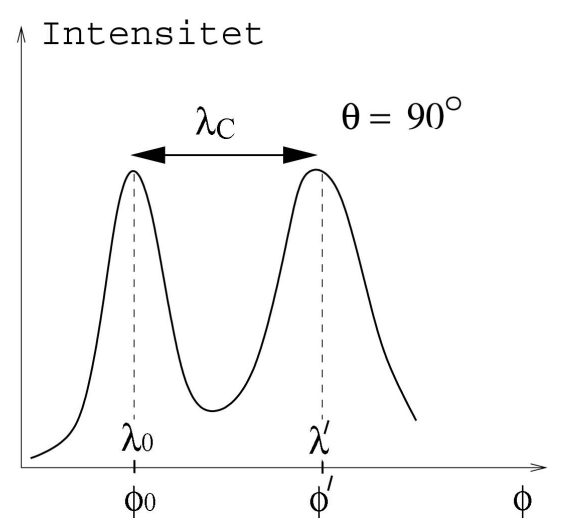
\includegraphics[width = \textwidth]{Compton_spredning.png}
  \caption{Compton spredning}
  \label{fig: Compton_spredning}
\end{figure}
Vi får en spredning av intensiteten til bølgene som samles om to topper. Jo høyre vinkel $θ$, jo høyere spredning. 

\subsection*{d)}
De viktigste fysiske prinsippene for beregning av bølgelengden $λ'$ er de Broglie relasjonen med $p = h /λ$ og bevaring av energi og bevegelsesmengde før og etter kollisjon

\subsection*{e)}
\[
λ' = 0.121 + \frac{h}{m_ec}(1 - \cos θ) = 0.121 \text{ nm} + \frac{1240  \text{ eVnm}}{0.511 \text{ MeV}}(1 - cos 90) 
\]
\[
λ' = 0.121 \text{ nm} + 0.0024 \text{ nm} = 0.123 \text{ nm}
\]

\subsection*{f)}
Noen av fotonene vil kollidere med elektroner som er løst bunnet til atomet. Dette modellerer vi som en kollisjon mellom fotonet og et elektron. Elektronets lave masse gjør at fotonet beholder mesteparten av energien etter kollisjonen. Noen andre fotoner kolliderer med elektroner sterkt bunnet til atomet. Disse modellerere vi som en kollisjon mellom fotonet og hele atomet. Her mister fotonet mye av sin energi, og får dermed økt bølgelengde. Da blir interferens mønsteret som resultat av Bragg-diffraksjonen litt annerledes og vi før en bølgetopp litt unna den til fotonene med lavere bølgelengde. Ettersom bevegelsesmengde må være bevart vil vi se størst forskjell i bølgelengden når $θ = 180^∘$, ettersom fotonene som kolliderer med hele atomet må endre retning fullstendig og miste mye energi.

\paragraph*{FASIT}
Toppen nær $λ_0$ skyldes at et foton har kollidert med et elektron det ikke har hatt nok energi til å løsrive elektronet fra atomet. Dermed må vi bergene atomets rekykleffekt (og ikke elektronets). Da må vi sette inn det massen til atomet istedet. 


\section*{Oppgave 2}
\subsection*{a)}
\paragraph*{Klassisk Partikkel}

Ved tilfelle der $E < V_0$ vil partikkelen alltid reflekteres tilbake. Når $E > V_0$ vil partikkelen alltid passerer barrieren. 

I en klassisk forståelse av fysikk er det fullstendig deterministisk hvorvidt partikkelen passerer barrieren eller ikke. 

\paragraph*{Kvantemekanisk Partikkel}
Ved tilfeller der $E < V_0$ er det en over 50\% sannsynlighet for at partikkelen partikkelen blir reflektert tilbake. Når $E > V_0$ er det over 50\% sannsynlighet for at partikkelen passerer barrieren. 

I en kvantemekanisk forståelse av fysikk er det ikke deterministisk hvorvidt partikkelen passerer barrieren eller ikke. Ved endring av potensialet, vil det være en sannsynlighet for at partikkelen passerer barrieren. Jo høyere potensialet, jo lavere sannsynlighet for passering. 


\subsection*{b)}
% TODO: Undersøk skissen her. Skal bølgelengden øke når potensialet økter?


\section*{Oppgave 3}
\subsection*{a)}
$n$, $l$, og $m$ kalles kvantetallene og beskriver et elektron sin posisjon i et atoms orbitaler. Hovedkvantetallet $n ∈ ℕ$ beskriver hvilket hovedskall elektronet befinner seg i. Videre har vi $l ∈ [0, n-1]$. Tallet beskriver størrelsen på angulærmomentet og beskriver formen på skallet. Dette noteres gjerne med  s, p, d og f. Videre har vi $m_l ∈ [-l,l]$, som beskriver størrelsen på angulærmomentet i z-retning. Dette bestemmer hvilken orbital elektronet tilhører. Det er plass til 2 elektroner i hver orbital. Én med spin $1 / 2$, og én med spin $-1 / 2$.

\subsection*{b)}
Vi løser følgende likning. Normerisngsintegralet må være i 3 dimensjoner
\[
∫_{-∞}^{∞} ψ_{100}^{*} ψ_{100} \ \mathrm{d}r = A^2∫_{-∞}^{∞} e^{-2r / a} \ \mathrm{d}^3r = 1
\]

Vi må gjøre om til kulekoordinater. 
\[
∫_{0}^{π} ∫_{0}^{2π} ∫_{0}^{∞} A e^{- r / a}r^2 \sin θ \ \mathrm{d}r \ \mathrm{d}ϕ \ \mathrm{d}θ = 1
\]
\[
2πA^2 ∫_{0}^{π} ∫_{0}^{∞} r^2 e^{-r / a} \sin θ \ \mathrm{d}r \ \mathrm{d}θ = 1
\]
\[
4πA^2 ∫_{0}^{∞} r^2 e^{-r / a} \ \mathrm{d}r = 1
\]
Vi bruker at $∫_{0}^{∞} x^{n} e^{- x / a} \ \mathrm{d}x = n! a^{n + 1}$ for å løse integralet. Vi setter $x = 2r$ som gjør om integralet og bruker substitusjon. 

\[
4πA^2 \frac{1}{8} ∫_{0}^{∞} r^2 e^{-r / a} \ \mathrm{d}r = \frac{1}{2} πA^2 2! a^3 = 1
\]
\[
A = \sqrt{\frac{1}{πa^3}}
\]


\subsection*{c)}
Ettersom $n=1$ vet vi at $l=0$ og $m_l=0$ som dermed gjør at angulærmommentet er null. Dette er ikke overraskende ettersom vi har en sfærisk symmetrisk s-orbital.


\subsection*{d)}
\[
\hat{H} ψ_{1} = E_1 ψ_{1}
\]

Ettersom vi har en sfærisk symmetri og dermed angulærmoment null, vet vi at $\hat{L}^2 ψ = 0$ og vi kan dermed forkaste dette leddet. 
\[
- \frac{ℏ^2}{2m} \left(\frac{∂^2 }{∂ r^2} + \frac{2}{r} \frac{∂ }{∂ r}\right)ψ_1 - \frac{k}{r}ψ_1
\]
\[
- \frac{ℏ^2}{2m}\left(\frac{1}{a^2} - \frac{2}{ra}\right)A^{- r / a} - \frac{k}{r}A^{- r/ a} = E_1 Ae^{- r / a}
\]
Ettersom likningen skal stemme for alle $r$ løser vi for alle $r$-sammenhenger hver for seg. 
\[
E_1 = - \frac{ℏ^2}{2ma^2}
\]
Videre løser vi for de lineære $r$-sammenhengene. 
\[
\frac{ℏ^2}{2m} \frac{2}{ra} = \frac{k}{r} ⇒ a = \frac{ℏ^2}{mk} 
\]
\[
a = \frac{4πϵ_0ℏ^2}{me^2}
\]



\subsection*{e)}
Vi løser scrhödingerlikningen. 
\[
\hat{H} ψ_{1} = E_1 ψ_{1}
\]
\[
\left(- \frac{ℏ^2}{2m} \left(\frac{∂^2 }{∂ r^2} + \frac{2}{r}\frac{∂ }{∂ r} - \frac{\hat{L}^2}{h^2r^2}\right) - \frac{k}{r}\right) R_n(r)\sqrt{\frac{3}{4π}}\sin θ \sin ϕ
\]
  



\end{document}